\documentclass{article}
\usepackage{tjark_sty}
\usepackage{times,graphicx}
\usepackage{float}
\usepackage{subfigure}
%\usepackage{hyperref}
\usepackage{url}
\usepackage{amsmath}
\usepackage{amssymb}
\usepackage[small,tight]{bibhacks}
\nipsfinalcopy
%\documentstyle[nips14submit_09,times,art10]{article} % For LaTeX 2.09


\title{Team Description Paper of TJArk@Home}
%\title{Machine Translation with Recurrent Neural Networks}
% 

\author{
He Zongtao \\
Robot and Artificial Intelligence Lab\\
Tongji University \\
\texttt{1930719@tongji.edu.cn} \\
\And
Zhou Xun \\
Robot and Artificial Intelligence Lab\\
Tongji University \\
\texttt{1930719@tongji.edu.cn} \\
\And
Xu Weihan \\
Robot and Artificial Intelligence Lab\\
Tongji University \\
\texttt{1930719@tongji.edu.cn} \\
}




% The \author macro works with any number of authors. There are two commands
% used to separate the names and addresses of multiple authors: \And and \AND.
%
% Using \And between authors leaves it to \LaTeX{} to determine where to break
% the lines. Using \AND forces a linebreak at that point. So, if \LaTeX{}
% puts 3 of 4 authors names on the first line, and the last on the second
% line, try using \AND instead of \And before the third author name.

\newcommand{\fix}{\marginpar{FIX}}
\newcommand{\new}{\marginpar{NEW}}

%\nipsfinalcopy % Uncomment for camera-ready version

\begin{document}


\maketitle

\begin{abstract}

    RoboCup@Home is one of the world largest robotics competition aims at bringing robotic platforms to use
    in realistic domestic environments. 
    Although the competition has been held for years and many teams contributed a lot, there are still obstacles in service robotics technology, such as precise grasping, real-time object detection, etc.
    As to Social Standard Platform League with the Pepper platform, some tasks become more difficult due to limited hardware performance.
    In this paper, we describe our team's work on this competition and outline functions we have implemented on Pepper.
    Our software framework is homemade, including high-level package of native NAOqi API, ROS-based components, application skills and HTTP communication mechanism.
    We develop visual-SLAM and real-time naviagtion modules based on ROS and RTAB-Map. 
    Cameras and deep learning are used to deal with environmental reasoning and interaction tasks.
    There are also many interesting applications, such as conversation, action imitation.
    Finally, we designed a user-friendly GUI on Pepper's pad, so that any amateur can control the robot and enjoy its service.
    When we first took part in China RoboCup@Home competition in 2019, we won the first-place. 
    We are eager to do more and show more on a broader stage.


\end{abstract}


\section{Introduction}
As development of robotic technology, more and more people expect intelligent robots to serve the family as human beings and provide a good and comfortable life experience. The RoboCup@Home competition \cite{inproceedings} focus on bringing robotics to apply in common domestic environment. To achieve such goal, the robotic system must be able to perceive environment, communicate with humans and complete various tasks, such as cleaning up a table, holding a party or guiding new comers. Security is the top priority. Because service robots can't do harm to people and the environment. Secondly, the robot should be controllable. The operator can intervene the behavior of the robot at any time to prevent the unexpected situation. Finally, the robot should have complete autonomous action ability and give people comfortable interaction experience. 

The Robotics and Artificial Intelligence Lab (RAIL) of tongji university was founded in 1992, Team TJArk of RAIL was founded in 2004 and participated in RoboCup World Cup from 2006 to 2018. We have got seven winning streak in China RoboCup SPL and once won the third place in RoboCup2018 SPL.
In December 2018, we founded an energetic new team to participate in RoboCup @Home League, called TJArk@Home. Main goal of TJArk@Home is to explore the limit of how well can robots serve people during common life with acceptable cost. Under the guidance of such wish, we are doing many research on the Pepper platform, such as
\begin{itemize}
\item SLAM(Simultaneous Localizaiton and Mapping)
\item Auto navigation of robot
\item Object Detection and Recognition
\item Human-face detection and analysis
\item Human-Robot interaction
\item Motion control
\item Trajectory teaching
\item Design of laptop GUI
\item ...
\end{itemize}
April 2019,  the first time TJArk@Home involved in China RoboCup@Home League, we got the first-place in SSPL(Social Standard Platform League). 
During the competion, we show a lot of abilities, including 
Autonomous navigation, 
Follow an operator to the given position, 
Recognize speech and response, 
Detect humans in vision and summarize their features. 

Although our team has not been established for a long time, we have developed a reusable and extensible software framework. 
It is a higher level integration of NAOqi API, which makes developing a new application more easily. 
The HTTP-based Information Exchange System(HIES) also helps a lot. 
Tasks require large computational resources such as syntactic analysis can be allocated to a host server. 
Pepper just need seed raw data and listen for response. Such mechanism reduce Pepper’s burden, allowing it pay more attention to interaction logic and task excution. 

Tongji RAIL lab has been researching on robotics since its begining, and achieved a lot in several aspects, such as humanoid walking \cite{rebalancecontrol}. ??. 
RoboCup@Home League is a new attempt, which involves former research ??, but bringing untouched challenges ??. 
We are pushing researchs on vision, navigation, interaction and building a simulated competition scenario for integration testing.


\section{Architecture}
\label{sec:architecture}

As shown in \ref{fig:archi}, we have developed a Python framework, which is a high-level package of NAOqi APIs and ROS-based components. 
\begin{figure}[!h]
    \centering
    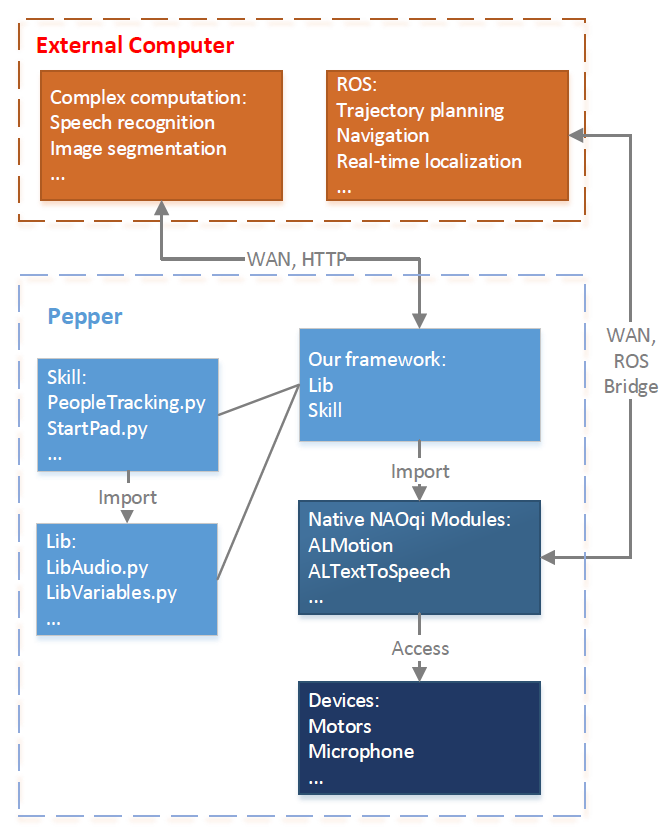
\includegraphics[width=4in]{figs/architecture.png}
    \caption{System architecture}
    \label{fig:archi}
\end{figure}

\subsection{NAOqi Operation System}
\label{subsec:naoqi}
In most aspects, NAOqi OS behaves like a Linux.
The most significant feature is its NAOqi modules.
Various modules can be accessed through network by the proxy called "ALBroker".
To upper level application, the proxy is transparent, which makes remote access has no difference with local access.
All underlying hardware can be used by these NAOqi modules easily.
\ref{fig:naoqi} shows the NAOqi architecture.

\begin{figure}[!h]
    \centering
    \subfigure[File organization]{\label{fig11}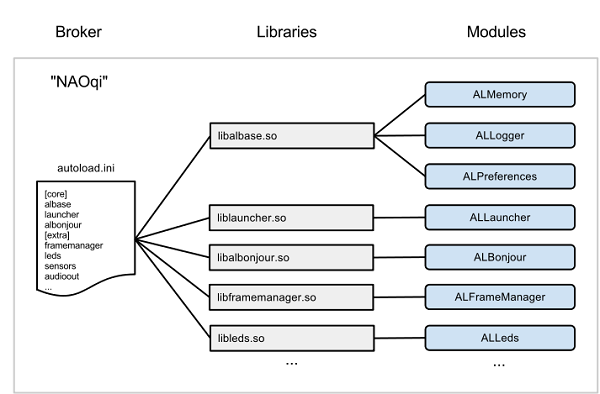
\includegraphics[width=2.5in]{figs/naoqi1.png}}
    \hspace{0.2in}
    \subfigure[Access process]{\label{fig12}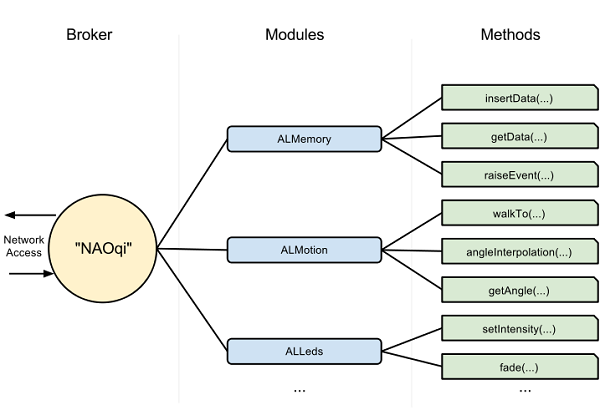
\includegraphics[width=2.5in]{figs/naoqi2.png}}
    \caption{NAOqi API}
    \label{fig:naoqi}
\end{figure}

\subsection{Homemade framework on Pepper}
\label{subsec:native}

On NAOqi OS, several processes are simultaneously running, including UI process, HTTP server/client process, motion control process, vision process, navigation process, etc.
All codes are organized into two main parts: libraries and skills. 
Libraries, we name them with “/Lib.*\.py/” pattern, are files that contain various class definitions for basic ablilities. 
Every “Lib” attaches to some specific functions. 
For example, “LibVariables” defines a class related to global variables stored on local disk or remote server. 
“Lib”s are just useful tools without any task-oriented purpose. 

To combine them together and implement specific applications, we write many app files, called “Skill”. 
A “Skill” imports several “Lib”s, to accomplish a complete task, such as tracking a person. 
Every “Skill” runs as an individual process, so communication problem follows. 
OS’s memory manager allocate different storage space for different processes, so there is no native global space for our different “Skill” and “Lib”. 
But most of time, there is a large need for them to share information. 
To overcome such dilemma, we developed a JSON-based global variable mechanism. As mentioned before, this function is implemented in “LibVariables”. 
It uses hard-disk to store a global variable with JSON format. 
Thanks to separation principle of interface and implementation, the global space can be not only Pepper local disk, but also remote server memory/disk. 

Overall, though many programs engaged, we just need to run a single shell script to start all applications we need. 
This native software system on Pepper is easy to learn, easy to use and easy to extend. 
Every team member can write his/her own lib files, such as "LibMoiton", "LibDetection", and add it to the framework by pushing their files to Pepper. 
The development process seems like building. It starts from a basic frame, and grows with bricks added by team members, and finally become a useful building.

\subsection{HTTP-based Information Exchange System}
\label{subsec:http}
Computational resources are limited in NAOqi OS. 
But in real applications quite a lot tasks need heavy computation, which require us to push them to a powerful remote computer.
So, we designed a HTTP-based information exchange system. There are two HTTP server process, one in Pepper, another in external computer. 

Main function of external computer server process is to listen to Pepper’s requests, start corresponding computing program and response the result to Pepper. 
A conspicuous example is speech recognition task. 
After recording a complex speech sentence from the operator, Pepper sends the audio file to the external computer through HTTP request. 
The computer receives this request, and converts this speech to text. 
Finally, speech text is sent back carried by HTTP response package. 

On the other hand, HTTP server process runs on Pepper mainly aims at web service. 
It contains a web site backend. 
When a browser login the URL, it gets a home page of various applications and can start them by simple clicks. 
Moreover, a device just need the ability of sending HTTP requests to control Pepper’s behavior. 
This part will be described at ?? in detail. 

The advantage of HTTP information exchange is obvious, it is widely used and device/language independent. 
But network quality would limit the performance of HTTP communication. 
Future works contain compressing information to reduce transfer load.

\subsection{Robot Operation System (ROS)}
\label{subsec:ros}

Implementing SLAM and auto-navigation of robot needs well fusion of multi-sensor data and feedback control of motion actuators, so Robot Operating System (ROS) is a useful tool. 
We develop a basic module serving as a bridge between NAOqi and ROS, it publish Pepper’s sensor data in ROS format and enable ROS to call NAOqi’s APIs. 
ROS components get multi-sensor data, then do SLAM and path planning with real-time obstacle avoidance. 
As a result, motion commands will be sent to NAOqi.

\section{Vision Simultaneous Localization and Mapping (VSLAM)}
\label{sec:vslam}

Pepper needs a model (a map) of the environment to support other tasks, mainly auto-navigation, but a prior map is often not available in various home scenarios, so SLAM find its application. 
The stereo camera data is mainly used by a visual SLAM module, together with laser (very limited) and odom (has significant error) data. 
Our VSLAM algorithm is based on RTAB-Map, a graph-optimized based VSLAM algorithm, and have been modified for Pepper's sensors. 
Odom and laser scan data make the initial pose estimation, then stereo data serves for appearance-based loop closure detection to optimize local and global pose. 
VSLAM can get a 3D point cloud, we make a projection to get a 2D grid map for navigation. 
Having map and Pepper’s size parameters, we use DWA (Dynamic Window Apporach) to plan the path and fuse vision, laser and sonar data to make real-time obstacle avoidance (mainly for dynamic scene), a series of motion command will be sent to NAOqi APIs, so Pepper can navigate to its goal points itself.

\begin{figure}[h]
    %\centerline{    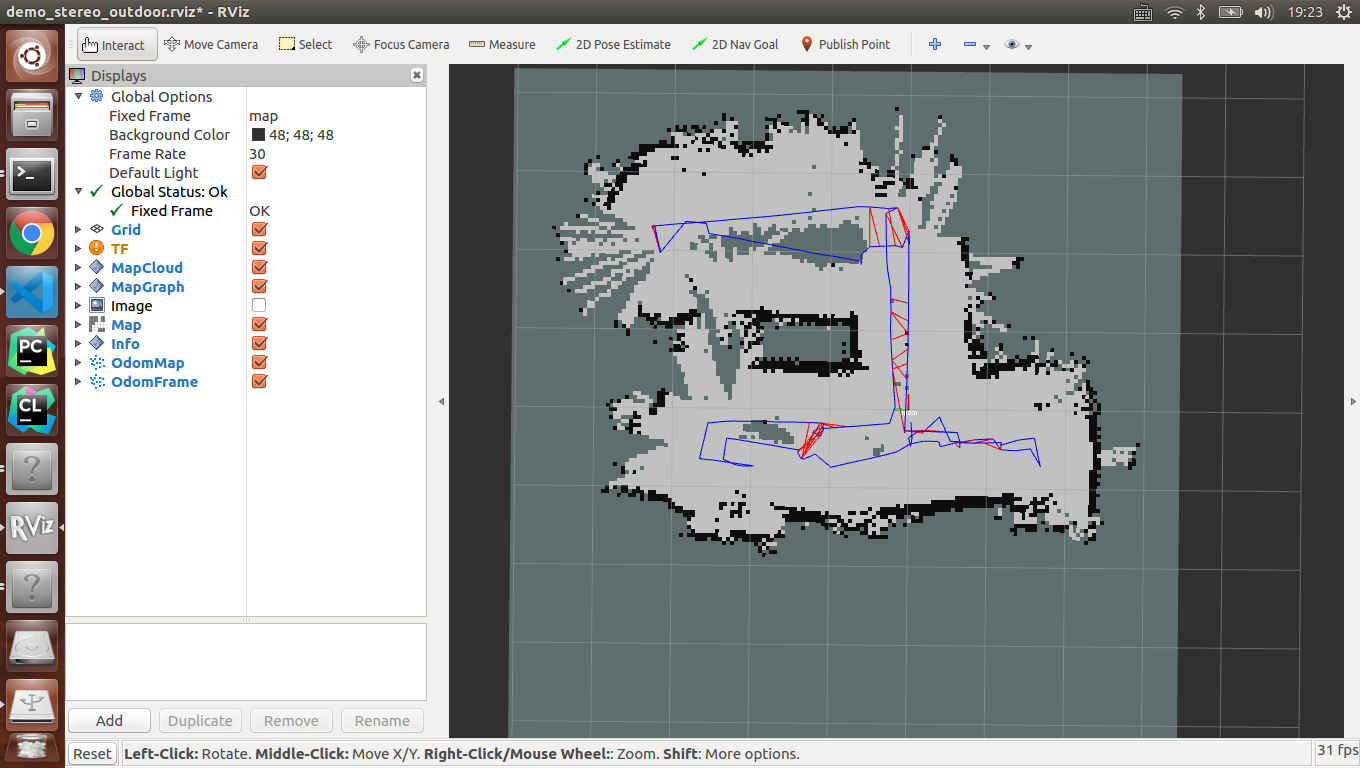
\includegraphics[width=1.\textwidth]{figs/vslam_shortcut.png} }  
    \centering
    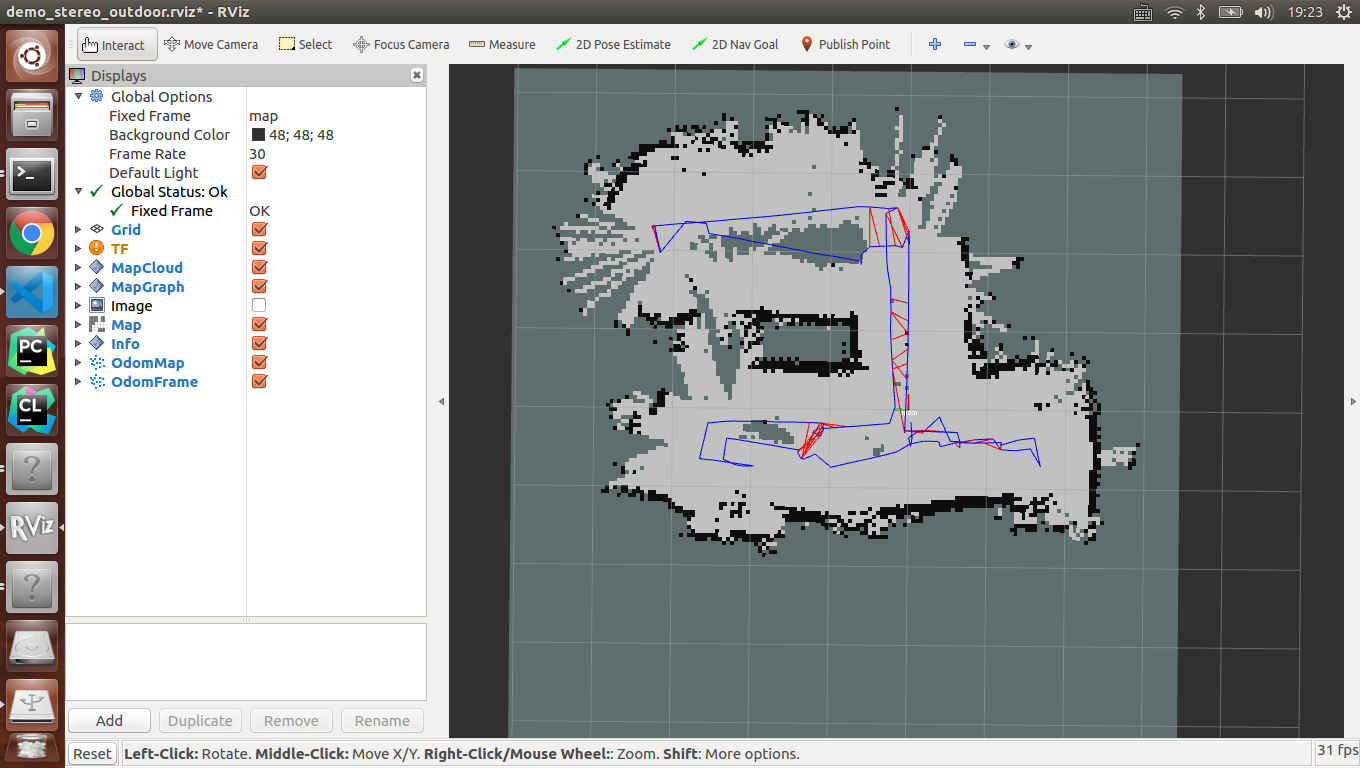
\includegraphics[width=1.\textwidth]{figs/vslam_shortcut.png}
    \caption{SLAM and navigation on ROS}
    \label{fig:vslam}
\end{figure}

\section{Computer Vision}
\label{sec:vision}
Various vision algorithms are needed for more careful perception and analysis of Pepper's environment pn object and huamn level. 
To start interaction, our Pepper can detect and recognize different people, remember their names and some other features, and track them using its camera data. 
Then, more interested skills will be shown to carry more complex tasks. For example, some tasks require human posture recognition so an alogorithm based on OpenPose \cite{Cao_2017_CVPR} is developed. 
It can recognize human skeleton so that we can judge whether a person is standing, sitting or pointing somewhere. For object-level environment reasoning, a detection and recognition framework based on YOLOv3 \cite{Redmon2018YOLOv3AI}, which is an object detection algorithm based on CNN.
According to the competition environment of RobCup@Home, our object detection system can detect 50 classes of indoor objects in real time and print its name in the figure.
To train our object detection network, we made a dataset containing 50 classes indoor objects from OpenImages.We also matched adjacent input frames to increase the robust of detection.
In some detection tasks need a large field of view, but the top 2D camera has a limited view. So we need to take some measures to expand the Filed of view.
The method we choose is stitching images getting from different perspective,to decrease the influence of light change or deformation,we then use fusion algorithm. This method can improve the comprehensive of detection .
\begin{figure}[h!]
\centering
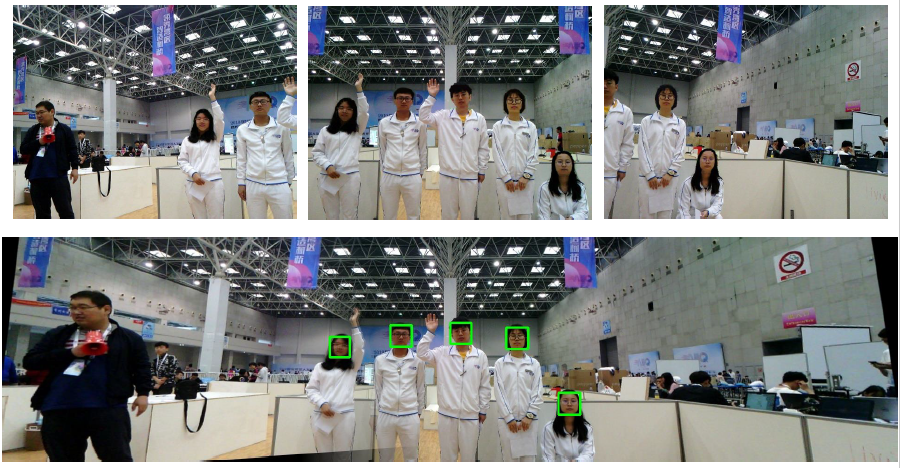
\includegraphics[width=1.\textwidth]{figs/vision1.png}
\caption{Image Stitch and Fusion to Detect in a Lager Field of View}
\label{fig:vision1}
\end{figure}
Now we are trying to expand the visual functions like person's pose estimation. 
For person's pose estimation,we use OpenPose model to perform multi-person pose estimation. 
The main steps of this method are input image stream, predict confidence map for body part detection and vector fields of part affinities, then clustering the key points to matching associate body parts, and finally assemble them into full body pose in image. 
\begin{figure}[h!]
    \centering
    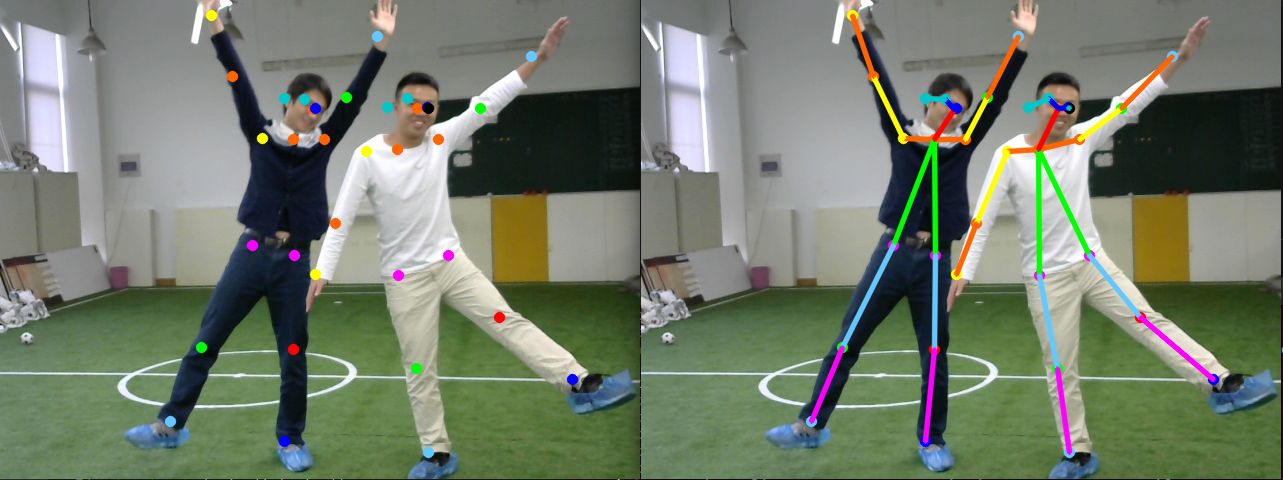
\includegraphics[width=1.\textwidth]{figs/vision2.png}
    \caption{Using OpenPose model to estimate body pose}
    \label{fig:vision2}
    \end{figure}

The Naoqi framework contains many useful APIs,so we take advantages of them. 
For vision part,we can use API to judge person whether standing or sitting, whether close or far away from robot. 
They can also analyze person's expression and clothes color. These functions are integrated to human-robot interaction module.

\section{Human-Robot Interaction}
\label{sec:hri}

\subsection{Graphics User Interface}
\label{subsec:gui}
As a domestic service robot, smooth GUI interaction is neccesary. 
One of the advantages of Pepper is that it has a laptop on its breast, which makes GUI possible. 
We designed a user-friendly and cross-platform interface so even people unfamiliar to robotics can quickly operate on Pepper. 

We have put twenty applications on the GUI so far, including Motion, Conversation, Vision, Joints, etc. 
In Motion, the operator can make the robot move a given distance to a given direction, or just move by a constant velocity.
In Conversation, the operator can chat with Pepper using English or Chinese.
In Vision, camera information is integrated. All images Pepper captured will be displayed here and the resolution is modifiable.
In Joints, all joints' status are listed for developer to debug.
We wish such GUI can help Pepper more powerful and useful.

\begin{figure}[!h]

    \centering
    \subfigure[Home page]{\label{fig11}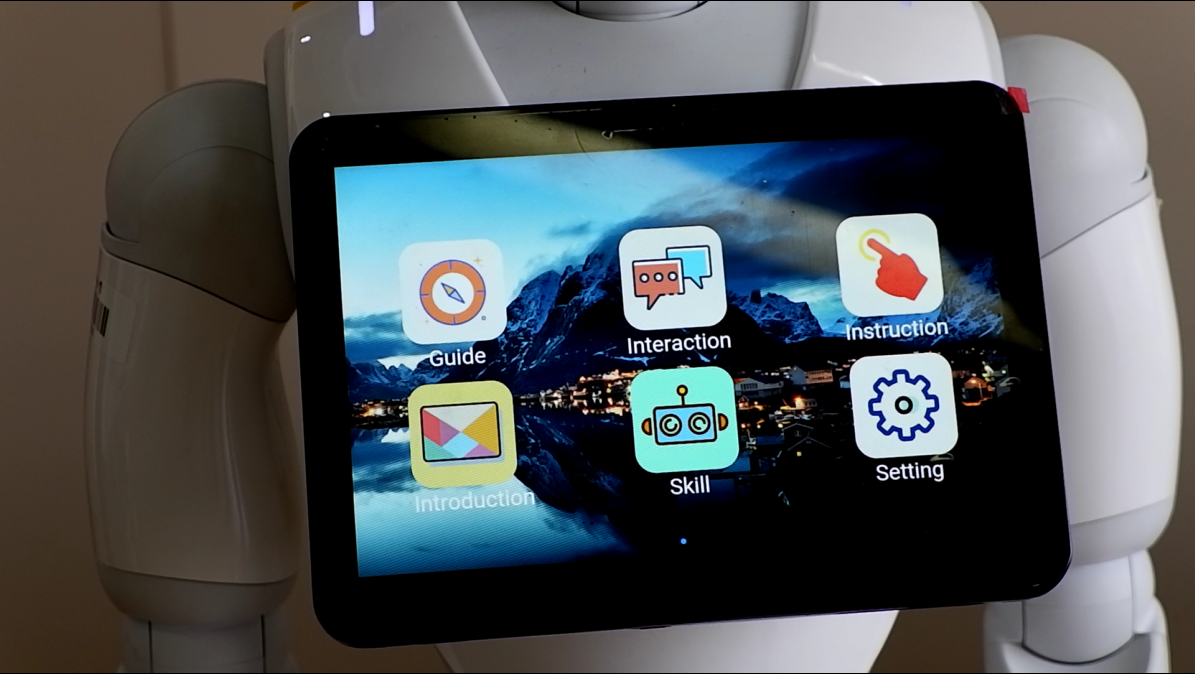
\includegraphics[width=2.5in]{figs/gui1_1.png}}
    \hspace{0.2in}
    \subfigure[Vision page]{\label{fig12}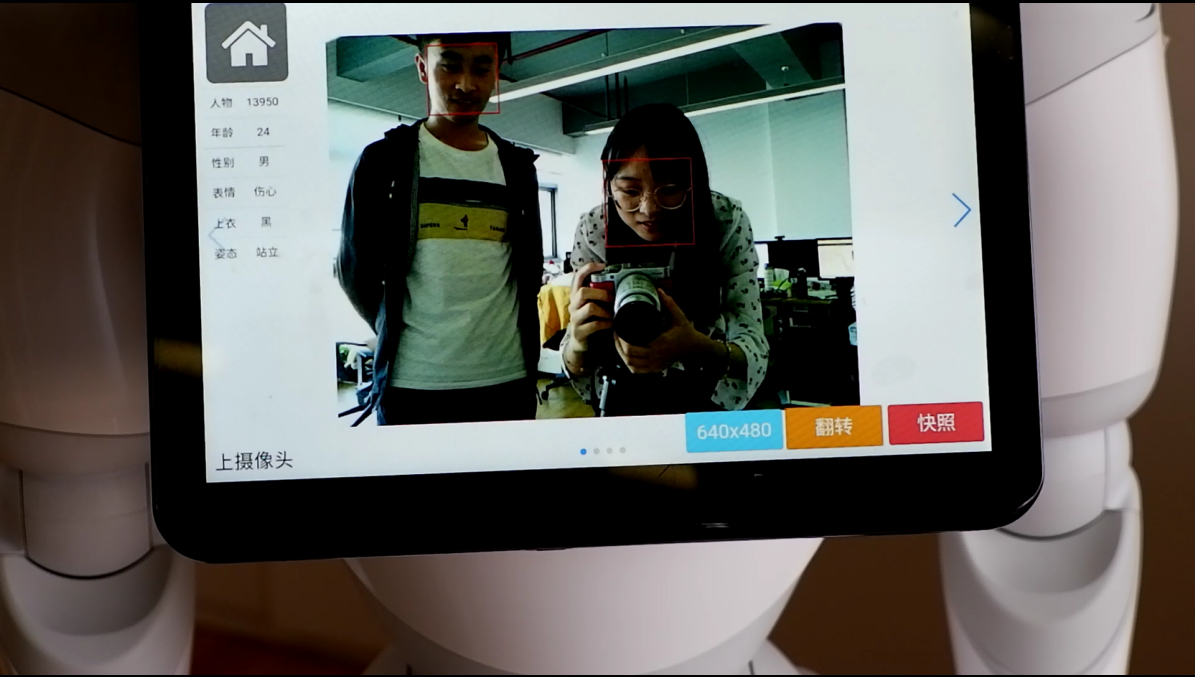
\includegraphics[width=2.5in]{figs/gui1_2.png}}\\
    
    \subfigure[Depth image page]{\label{fig13}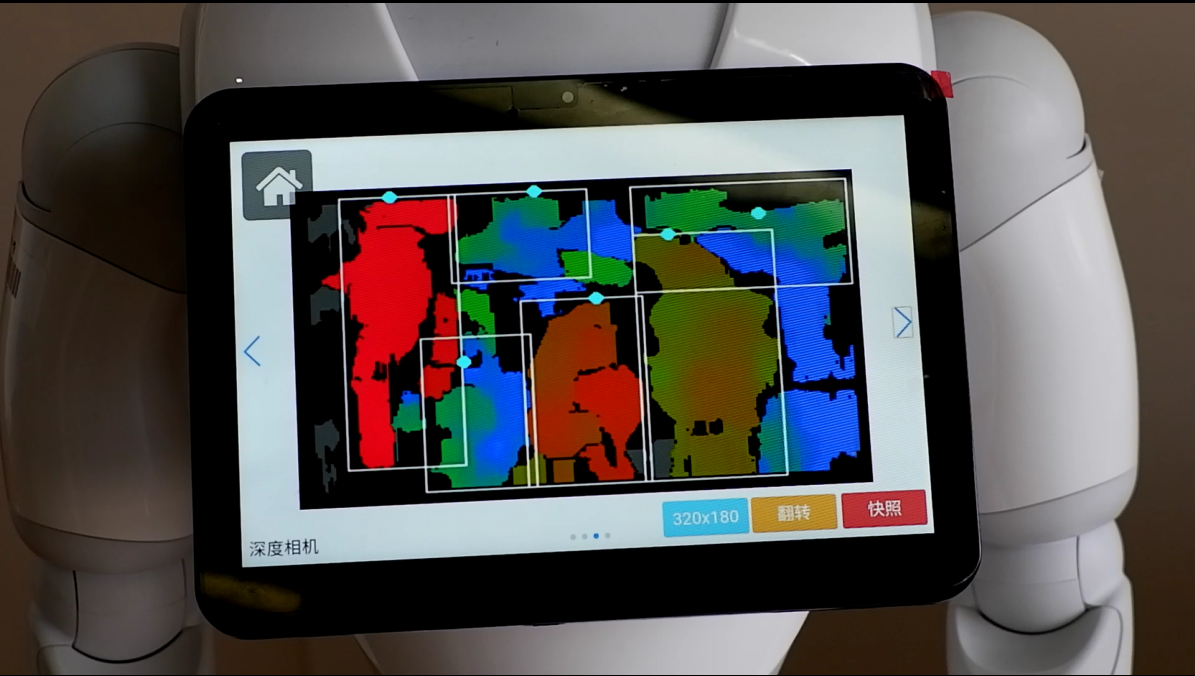
\includegraphics[width=2.5in]{figs/gui1_3.png}}
    \hspace{0.2in}
    \subfigure[Joints page]{\label{fig14}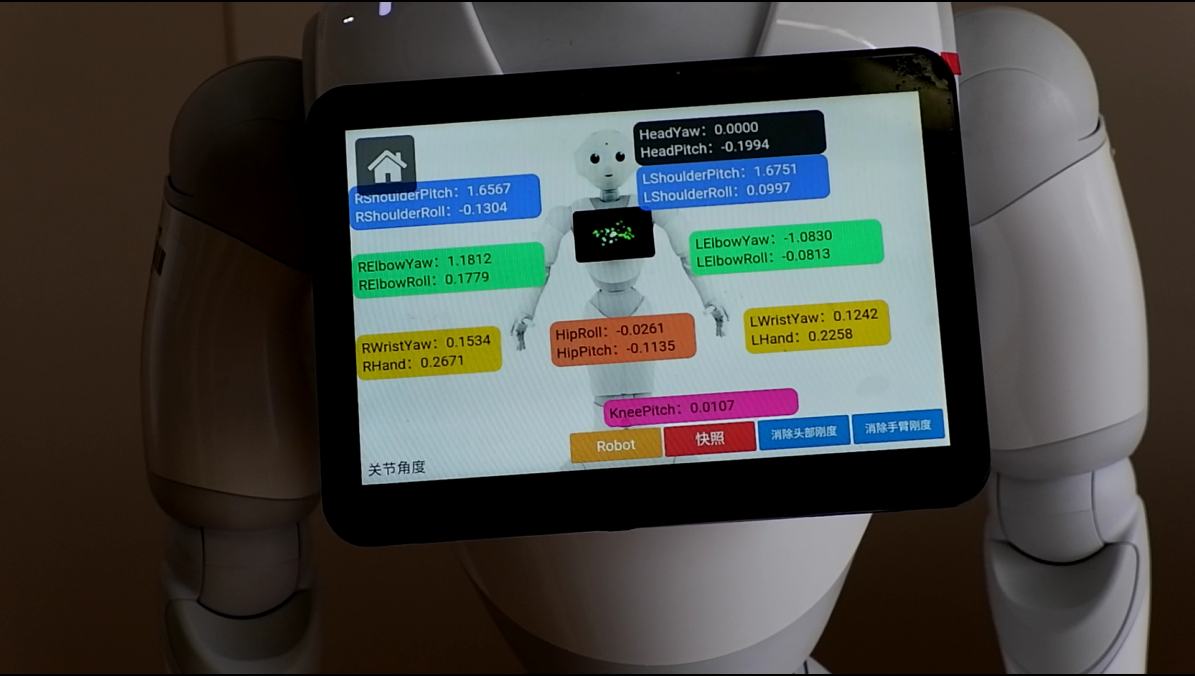
\includegraphics[width=2.5in]{figs/gui1_4.png}}

    \subfigure[Action teaching page]{\label{fig15}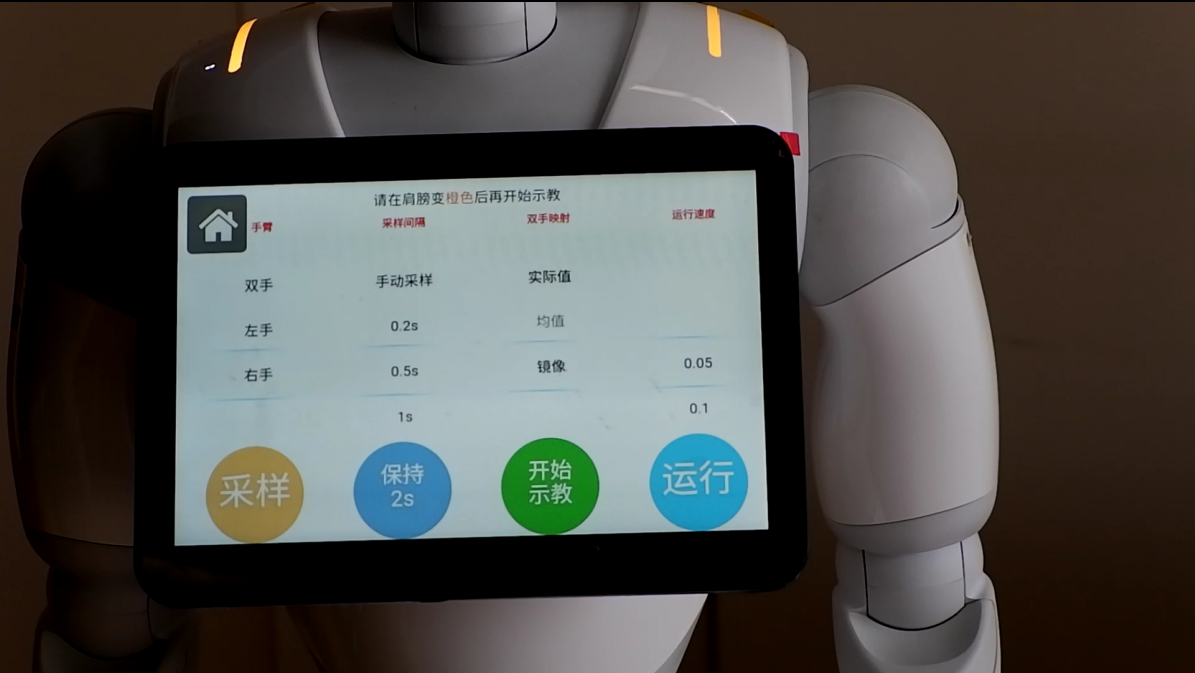
\includegraphics[width=2.5in]{figs/gui1_5.png}}
    \hspace{0.2in}
    \subfigure[Conversation page]{\label{fig16}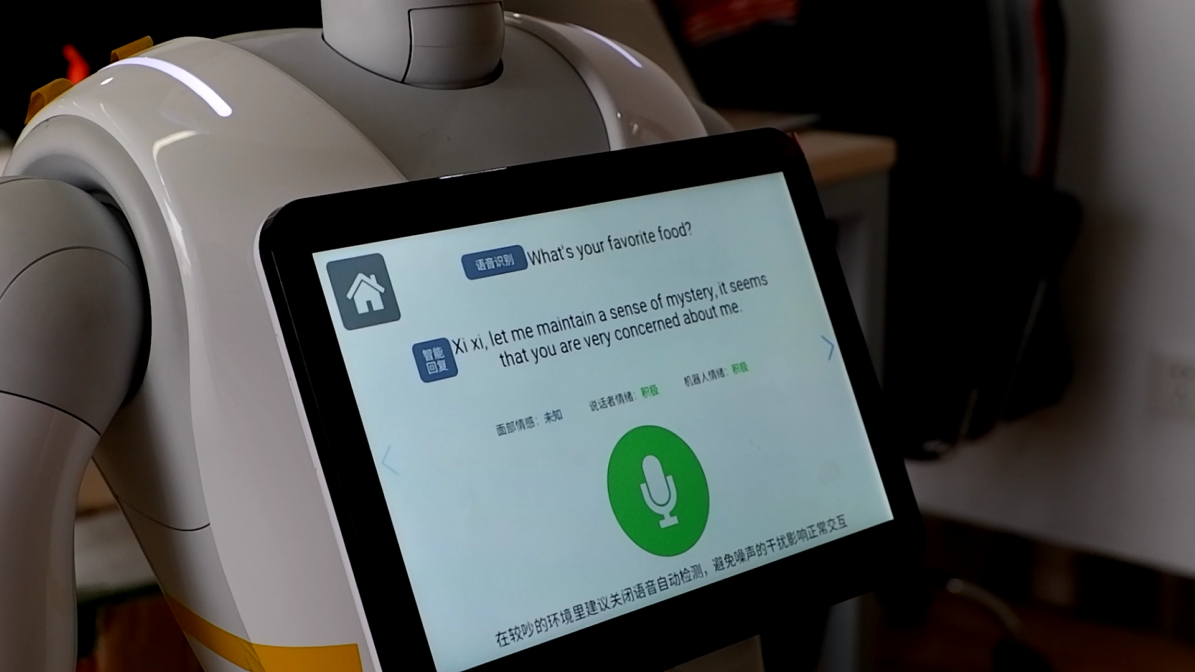
\includegraphics[width=2.5in]{figs/gui1_6.png}}


    \caption{GUI on Pepper's pad}
    
    \label{figb} %% label for entire figure
    
    \end{figure}

\subsection{Speech Interaction}
\label{subsec:speech}
As mentioned in \ref{subsec:gui}, we develop a conversation function. 
Language is an important interaction way in daily life.
As a domestic service robot, it should have the ability to understand natural language.
Our conversation applicaiton is powered by Xunfei cloud speech engine.
The demonstration video has been uploaded to ??.
However, this function is triggered by pad touch, which makes the chat not so less smooth.
We are trying to make Pepper can have the ability to understand natural language.

\subsection{Touch Interaction}
\label{subsec:otherinteraction}
To make Pepper more seem more smart, we develop some other interaction way to enrich its behaviors.
When a person touch its head, it would say something like "Huh, I feel a warm hand on my head".
And if Pepper's hand was grab, it will softly close hand and hold you, and greet you.
What's more, whenever pad or tactile sensors are touched, Pepper will look at that direction and speak or perform some body languages corresponding the condition.
Such touch interaction is funny and important.
It shows the robot is perceiving environment and ready to work.

For us developer, tactile sensors can do more.
There are three parallel tactile sensors on Pepper's head.
We designed a state machine to judge the touch direction.
If the touch is front to back, the head stiffness will be toggled.
If the touch is back to front, the arm stiffness will be toggled.
If the hand is touched more than 3 seconds, corresponding arm stiffness wil be toggled.
When we want to change some stiffness, we just need touch the robot rather than back to computer and run some codes.


\small
\section{Acknowledgments}

We thank Samy Bengio, Jeff Dean, Matthieu Devin, Geoffrey Hinton, Nal Kalchbrenner, Thang Luong, Wolfgang
Macherey, Rajat Monga, Vincent Vanhoucke, Peng Xu, Wojciech Zaremba,
and the Google Brain team for useful comments and discussions.


\bibliography{TJArk_TDP} 
\bibliographystyle{plain}

\newpage
\section{Team Information}
\label{sec:team}

\subsection*{Team Name}
TJArk@Home

\subsection*{Contact Information}
He Zongtao \\
Robot and Artificial Intelligence Lab (RAIL) \\
Tongji University \\
Caoan Road 4800, Jiading, Shanghai, China \\
1930719@tongji.edu.cn 

\subsection*{Website}
https://tjark.cn/file/Pepper/TJArk@Home/

\subsection*{Team Members}
He Zongtao, Xu Weihan, Zhou Xun, Liu Zhihao, Deng Xiuqi, \\
Wang Liuyi, Wang Naijia, Du Jiayuan, Lu Liwen

\subsection*{Description of Hardware}
Pepper by Softbank Robotics \\
Wireness Router \\
Server computer connected by WiFi \\

\subsection*{Description of Software}
Operation System: Ubuntu 18.04/16.04 LTS; NAOqi OS \\
Web Server: Tornado \\
Middleware: ROS \\
SLAM and Navigation: RTAB-Map, NAOqi driver \\
Object Recognition: YOLOv3 \\
Face Dtection and Recognition: YOLOv3 \\
Human Pose Estimation:  OpenPose \\
Speech Synthesis: Xunfei Cloud Service\\
Speech Recognition: Xunfei Cloud Service \\

\end{document}
